\chapter{InSAR技术原理}

\section{SAR与InSAR原理}

\subsection{SAR}
SAR由传统的雷达技术发展而来。
通过水平向和垂直向的压缩成像技术能够实现以较小的雷达天线
得到较高空间分辨率的影像。
每幅SAR影像的数据为光波从天线到地面每一个像素点然后反射再被天线接受的相位延迟。
即
\begin{equation}
    \phi=-\frac{4\pi}{\lambda}r
\end{equation}

\subsection{InSAR}
如果对于同一块区域有两幅影像,就可以对两幅影像做干涉处理。
原理如图\ref{fig:geometry}所示。
\begin{figure}[htb!]
    \centering
    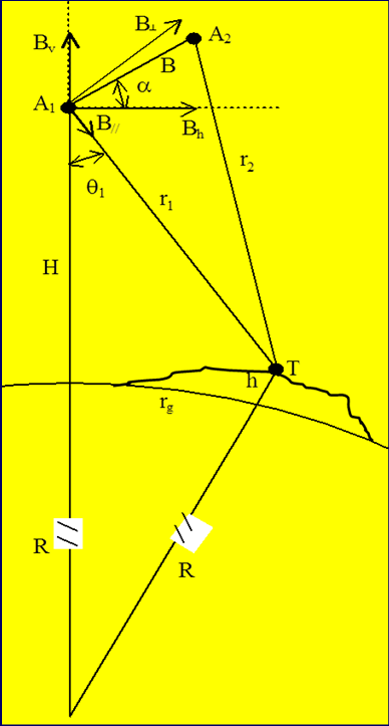
\includegraphics[width=0.5\textwidth]{geometry.png}
    \caption{InSAR技术原理示意图}
    \label{fig:geometry}
\end{figure}
所谓干涉,就是指二者相位相减。即
\begin{equation}
    \Delta \phi=-\frac{4\pi}{\lambda}(r_1-r_2)
\end{equation}
其中$r_1-r_2$为卫星视线方向的距离变化。
注意这里讨论的只是忽略大气效应即其他失相干效应,只考虑理想情况。
通常情况下,两幅影像并不是在相同的位置拍摄,二者之间有一定的距离。
所以当不存在任何的地表形变的情况下,可以通过一些几何的参数将此变化表达出来。
\begin{equation}
    \Delta \phi=\frac{4\pi}{\lambda}\left(\sqrt{r_1^2−2(B_hsinθ_1−B_{\perp}sinθ_1)r_1+B^2}−r_1\right)
\end{equation}

如果已知数字高程模型的话,可以算出来在理想条件下,无形变时的相位差。
将实际算得的相位差和无形变时理论计算的相位差相减,剩余的相位差即为因形变引起的相位差。
\begin{equation}
    \Delta \phi_{r}=-\frac{4\pi}{\lambda}u_{LOS}
\end{equation}
其中,$u_{LOS}$为地表形变在卫星视线(line-of-site:LOS)方向的投影,
从而可以把地表在卫星视线方向的形变算出来。
这种技术称之为D-InSAR。

注意,实际的到的相位是“缠绕”的相位,即相位是处于$(-\pi,\pi]$之间的。
将缠绕的相位通过解缠操作之后才得到上文中使用的相位。
解缠的方法很多,基本的假设是相邻像素的相位差不超过$\pi$。

诸多实例(火山喷发变形,地震震前和震后变形,地面沉降)
均证明InSAR是一种有效的测量地表形变的技术。

\section{PS-InSAR简介}
两幅SAR影像间隔时间可能很长,如果地表有植被,或者一年中有部分时间被冰雪覆盖,
地表散射体在这段时间内有较大的变化,有可能导致干涉图的失相干。
如果能挑出地表散射体中较稳定的部分,如建筑物,道路桥梁,岩石等
永久散射体(persist scatterer)反射波的相位差,剔除掉不稳定的散射体反射波的相位差,
经相位解缠之后就能得到较可靠形变结果。
这正是PS-InSAR技术的初衷。

2001年,Ferretti等人首次提出PS-InSAR技术。
即在一组时间序列SAR影像中选取相干性和稳定性均较好的永久散射体。
通过这些PS点的相位信息获得地表形变信息。
2004年,Andy hopper提出了新的PS算法,并将其实现在StamPS软件中\cite{hooperRecentAdvancesSAR2012}。
本研究使用这一软件获得形变信息。

PS-InSAR技术的主要内容为PS点的选取,分为两个步骤:
\begin{enumerate}
    \item 初步筛选。
    这一步通过分析模长的稳定性做筛选。
    Ferretti等人证明了,对于反射波的复信号,当相位的标准差较小时,有
    \begin{equation}
        \sigma_\varphi \approx \frac{\sigma_a}{\mu_a}
    \end{equation}
    其中,$\sigma_\varphi$是相位标准差,$\sigma_a$是模长的标准差,$\mu_a$是模长的均值。
    通过设置$\frac{\sigma_a}{\mu_a}$的上界$D_A$,筛选出一批PS点。
    \item 再次筛选。
    这一步通过分析相位的稳定性来做筛选。
    首先通过相位滤波得到噪声相位,对噪声相位做进一步的筛选选出最终的PS点。
\end{enumerate}

PS-InSAR的输入数据为连续的$M$幅SAR影像以及数字高程模型(DEM)。
首先,选取某一幅影像为主影像,然后通过配准,差分干涉,
以及PS点的选取等操作得到$M-1$幅干涉图,
之后通过相位解缠得到形变图以及平均形变速率图。

PS点的差分干涉相位中主要的误差来源于高程误差,大气影响等因素,每个PS点的相位组成可以表达成:
\begin{equation}
    \varphi_{diff}=\varphi_{topo}+\varphi_{def}+\varphi_{orb}+\varphi_{atm}+\varphi_{noise}
\end{equation}
其中
\begin{itemize}
    \item $\varphi_{topo}$为由于所采用的数字高程模型DEM不够准确而造成的误差,可以证明
    \begin{equation}
        \varphi_{topo}=-\frac{4\pi B_{\bot}}{\lambda R sin \theta}\epsilon
    \end{equation}
    \item $\varphi_{def}$为地表形变导致的差分干涉相位的变化,一般来说是研究所需要的结果,其余的各项均为误差;
    \item $\varphi_{orb}$是卫星轨道定轨不精确,轨道参数不准确引入的误差;
    \item $\varphi_{atm}$为大气的延迟效应导致的误差,由于光波在大气这种介质中的传播速度相对于真空中的光速有一定的偏差而引入这一误差;
    \item $\varphi_{noise}$为其他的一些噪声效应引入的误差,如热噪声等。
\end{itemize}

\section{SBAS-InSAR简介}
SBAS是另外一种利用多个SAR影像数据的时间序列InSAR方法。
SBAS通过设置选取SAR影像配对的时空基线的上限,
将所有的SAR影像分为了不同组,每组的基线较小,从而避免了空间上的失相干性,减小了失相干和高程模型误差的影响。

这里有必要简要叙述一下SBAS处理数据的算法。
假设一共有$n+1$景SAR影像数据,获取的时间分别为$t_0,t_1,\ldots,t_n$。
选取某一景影像为超级主影像。
满足时空基线限制的影响对共有$M$对。分别为$(A_1,B_1),(A_2,B_2),\ldots,(A_M,B_M)$。
则
\begin{equation}
    \Delta\phi_j=\phi_{A_j}-\phi_{A_j}
\end{equation}
其中,$j=1,2,\ldots,M$,$\phi_j$为第$j$景影像相对于超级主影像的差分相位,
$\Delta\phi_j$为第$j$组影像对的差分干涉相位,共计$M$个方程。
由已知的$\phi$根据以上方程求得$\Delta\phi$,
然后由得到的$\Delta\phi$反过来求$\phi$。
由于共有$M$个方程,$n$个未知数,方程组有无穷多组解,使用最小二乘法求最小二范数的解。

\section{StamPS软件简介}
StamPS是基于Matlab的一套软件,软件处理数据一共分为8步:
\begin{enumerate}
    \item 读取数据,并保存在matlab工作区;
    \item 估计相位噪声,这一步通过循环估计每一幅干涉图的每一个像素点的相位噪声;
    \item 通过分析各像素点的噪声情况筛选出PS点,这一步还估计出非PS点的像素的密度;
    \item 上一布只是粗略地选择PS点,其中还有较多的不稳定的像素点,这一步清除这些点;
    \item 去除所选择的像素点相位中空间不相关的视角误差;
    \item 相位解缠;
    \item 估计空间相关的视角误差,该误差绝大多数来源于空间相关的DEM误差,
    包括DEM本身的误差以及从地面坐标到雷达坐标投影的误差;
    \item 去除大气效应误差。
\end{enumerate}

\section{本研究所用的方法}
D-InSAR在监测地面沉降方面取得了一定的成果,但由于这种方法受失相干的影响比较严重,
并不适合本研究使用。
且由于数据较少的缘故,本研究采用StamPS中数据利用率更高的SBAS-InSAR\cite{hooperMultitemporalInSARMethod2008}方法处理数据。
